\subsection{Overview of MOSTWAS}

MOSTWAS incorporates two
methods to include distal-eQTLs
in transcriptomic prediction: mediator-enriched
TWAS (MeTWAS) and distal-eQTL prioritization
via mediation analysis (DePMA). 
As large proportions of total
heritable gene expression are explained
by distal-eQTLs local to regulatory
hotspots 
\cite{Liu2019,Pierce2014,Pierce2018Co-occurringMechanisms,Shan2019},
we used data-driven approaches
to either identify mediating
regulatory biomarkers (MeTWAS)
or distal-eQTLs mediated by 
local biomarkers (DePMA) to
increase predictive power and
power to detect gene-trait associations.
We assess in-sample predictive performance of MeTWAS and DePMA
via cross-validation over a user-defined $k$ folds
of training and test sets,
such that the expression model is estimated
in the training set and imputed into the test set
for cross-validation.
These
methods are summarized graphically
in \textbf{Figure \ref{fig:ch4_fig1}}.


\begin{figure}[!h]
	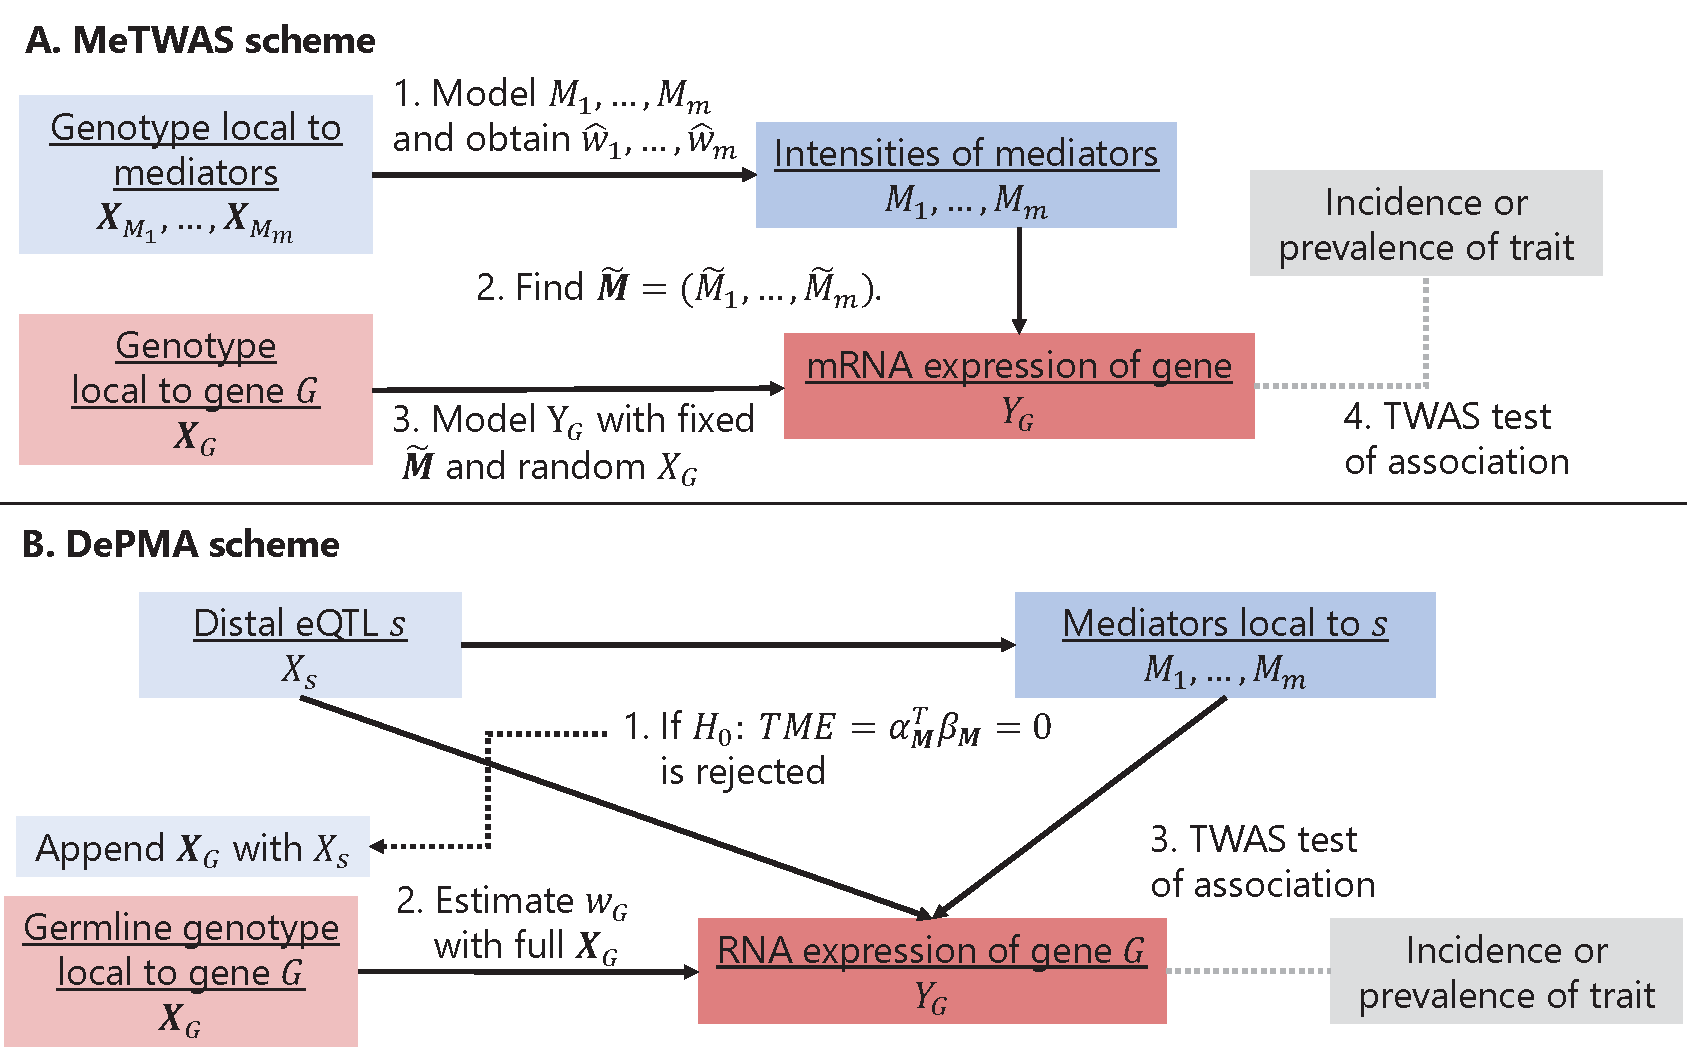
\includegraphics[width = \textwidth]{figures/ch4_fig1.pdf}
	\caption{\emph{Modeling schemes
	implemented in MOSTWAS.} (A) 
	Two-step least squares for mediator-enriched
	TWAS (MeTWAS). (B)
	Distal-eQTL prioritization by
	via mediation analysis (DePMA).}
	\label{fig:ch4_fig1}
\end{figure}

\begin{itemize}

\item MeTWAS first
identifies $m$ potential mediators
(e.g. CpG sites,
miRNAs, genes coding
for transcription
factors, etc) such
that the intensity (methylation, 
expression levels, etc) 
of these mediators are associated
with the mRNA expression of the gene of interest.
A model for the
genetically regulated intensities
(GRIn)
is estimated using
the local SNPs
to these mediators, and
the GRIn of these mediators
are imputed into the training
set.
The final gene expression model
is estimated by incorporating
the GRIn of the mediators
as fixed effects and 
the local SNPs 
to the gene as regularized
effects (see \textbf{Methods}
for more details).

\item DePMA
first identifies
testing triplets
of the gene of
interest, a distal
eSNP (SNP
in an eQTL) to the gene,
and any potential associated mediators local
to the eQTL. 
The total mediation effect (TME) 
of the eQTL on the gene 
through the set of mediators
is estimated
and the two-sided
hypothesis of $H_0: TME = 0$ is tested
via one of two options (\textbf{Supplemental
Figure \ref{fig:ch4_fig2}}).
Any distal-eSNP with a significant
TME is included with the SNPs
local to the gene of interest
to form the final design matrix.
A model including all
local SNPs and all significant
distal-eSNPs is fit to
the expression of the gene
using either elastic net
or linear mixed modeling (see \textbf{Methods}
for more details).

\end{itemize}

If individual genotype
data is available in
an external GWAS panel, using either
a MeTWAS or DePMA model, we impute expression
as a linear combination of the genotypes. If
only summary statistics are available
in the GWAS panel, the Imp-G weighted burden
testing framework \cite{Pasaniuc2014FastEnrichment},
as implemented in Gusev \etal \cite{Gusev2016},
can be applied. We further implement
a permutation test to assess whether
the overall association is significant
conditional on the GWAS effect sizes \cite{Gusev2016}
and an added-last test that assesses
the added information from distal-SNPs
given the weighted $Z$-score
from local SNPs (see \textbf{Methods} and \textbf{Supplemental
Materials}).

\subsection{Simulation analysis}

We first conducted simulations to assess
the predictive capability
and power to detect
gene-trait associations
under various settings
for phenotype heritability ($h^2_p$),
local heritability of expression ($h^2_{e,l}$),
distal heritability of expression ($h^2_{e,d}$),
and proportion of causal local ($p_{c,l}$)
and distal ($p_{c,e}$) SNPs
for MeTWAS and DePMA.
We considered two scenarios for each
combination of $(h^2_p, h^2_{e,l}, h^2_{e,d}, p_{c,l},
p_{c,e})$: (1) the leveraged association
between the distal-SNP and the gene of interest
exists in both the reference
and imputation panel, and (2) the leveraged association 
between distal-eSNP and the gene of interest
exists in the reference panel but does not contribute
to the heritable portion of the phenotype
in the imputation panel.
Using genetic data
from TCGA-BRCA, we used the 2,592 SNPs local to
the gene \emph{ESR1} 
on Chromosome 6 
to generate local eQTLs and
the 1,431 SNPs
local to the gene \emph{FOXA1}
to generate distal eQTLs for
a 400-sample eQTL reference panel
and 1,500-sample GWAS imputation
panel (see \textbf{Methods}).
Though the choice of these loci
was arbitrary for generating the simulated data, there
is evidence that \textit{ESR1} and 
\textit{FOXA1} are highly co-expressed in breast tumors
and local-eQTLs of \textit{FOXA1} have been
shown to be distal-eQTLs of \textit{ESR1} \cite{Guo2018AStudies}.

In these simulation studies, we found that
MOSTWAS methods performed well in
prediction across different
causal proportions and local and distal
mRNA expression heritabilities.
Furthermore, across all simulation
settings, we observed that MOSTWAS
showed greater or equal power
to detect gene-trait associations
as local-only models.
We found that, under
the setting that distal variation
contributes to trait heritability,
the best MOSTWAS model has greater power
to detect gene-trait associations
than the local-only model, with
the advantage in power over local-only
models increasing with increased distal
expression heritability (\textbf{Figure \ref{fig:ch4_fig3}A}).
Similarly, we found that as the proportion
of total expression heritability that
is attributed to distal genetic variation increased,
the positive difference in predictive performance
between the best MOSTWAS model and the local-only model
increased (\textbf{Supplemental Figure \ref{fig:ch4_suppfig1}}).
Under the ``null'' case that distal
variation influences expression
in the reference panel but
does not affect the trait in the GWAS panel,
we find that local-only and MOSTWAS models
perform similarly, as we would expect.
At low causal proportion
($p_c = 0.01$)
and low trait heritability ($h^2_p = 0.2$), 
local-only models have a
modest advantage in TWAS power over MOSTWAS models (shown
in \textbf{Supplemental Data}).
This difference is mitigated at larger
causal proportions and trait heritabilities
 (\textbf{Figure \ref{fig:ch4_fig3}B}).
 
 We also find that the power of
 the distal added-last increase significantly
 as both the sample sizes of the eQTL
 reference panel and the GWAS imputation
 panel increases. At
 a sample size of 10,000 in the GWAS panel 
 with summary statistics (a suitably
 large GWAS), we obtain
 greater than 65\% power to
 detect significant distal associations
 given the local association at
 eQTL sample sizes of greater than 200
 (\textbf{Supplemental Figure \ref{fig:ch4_suppfig4}}).
 Overall, these results demonstrated 
 the advantages of MOSTWAS methods for 
 modeling the complex genetic 
 architecture of transcriptomes, 
 especially when distal variation has a discernibly
 large effect on the heritability of both the gene 
 and trait of interest.
 Full simulation results are provided
 in \textbf{Supplemental Data} at
 \url{www.github.com/bhattacharya-a-bt/mostwas_paper}. The MOSTWAS
 package also contains functions
 for this simulation framework.

\begin{figure}[htbp]
\centering
	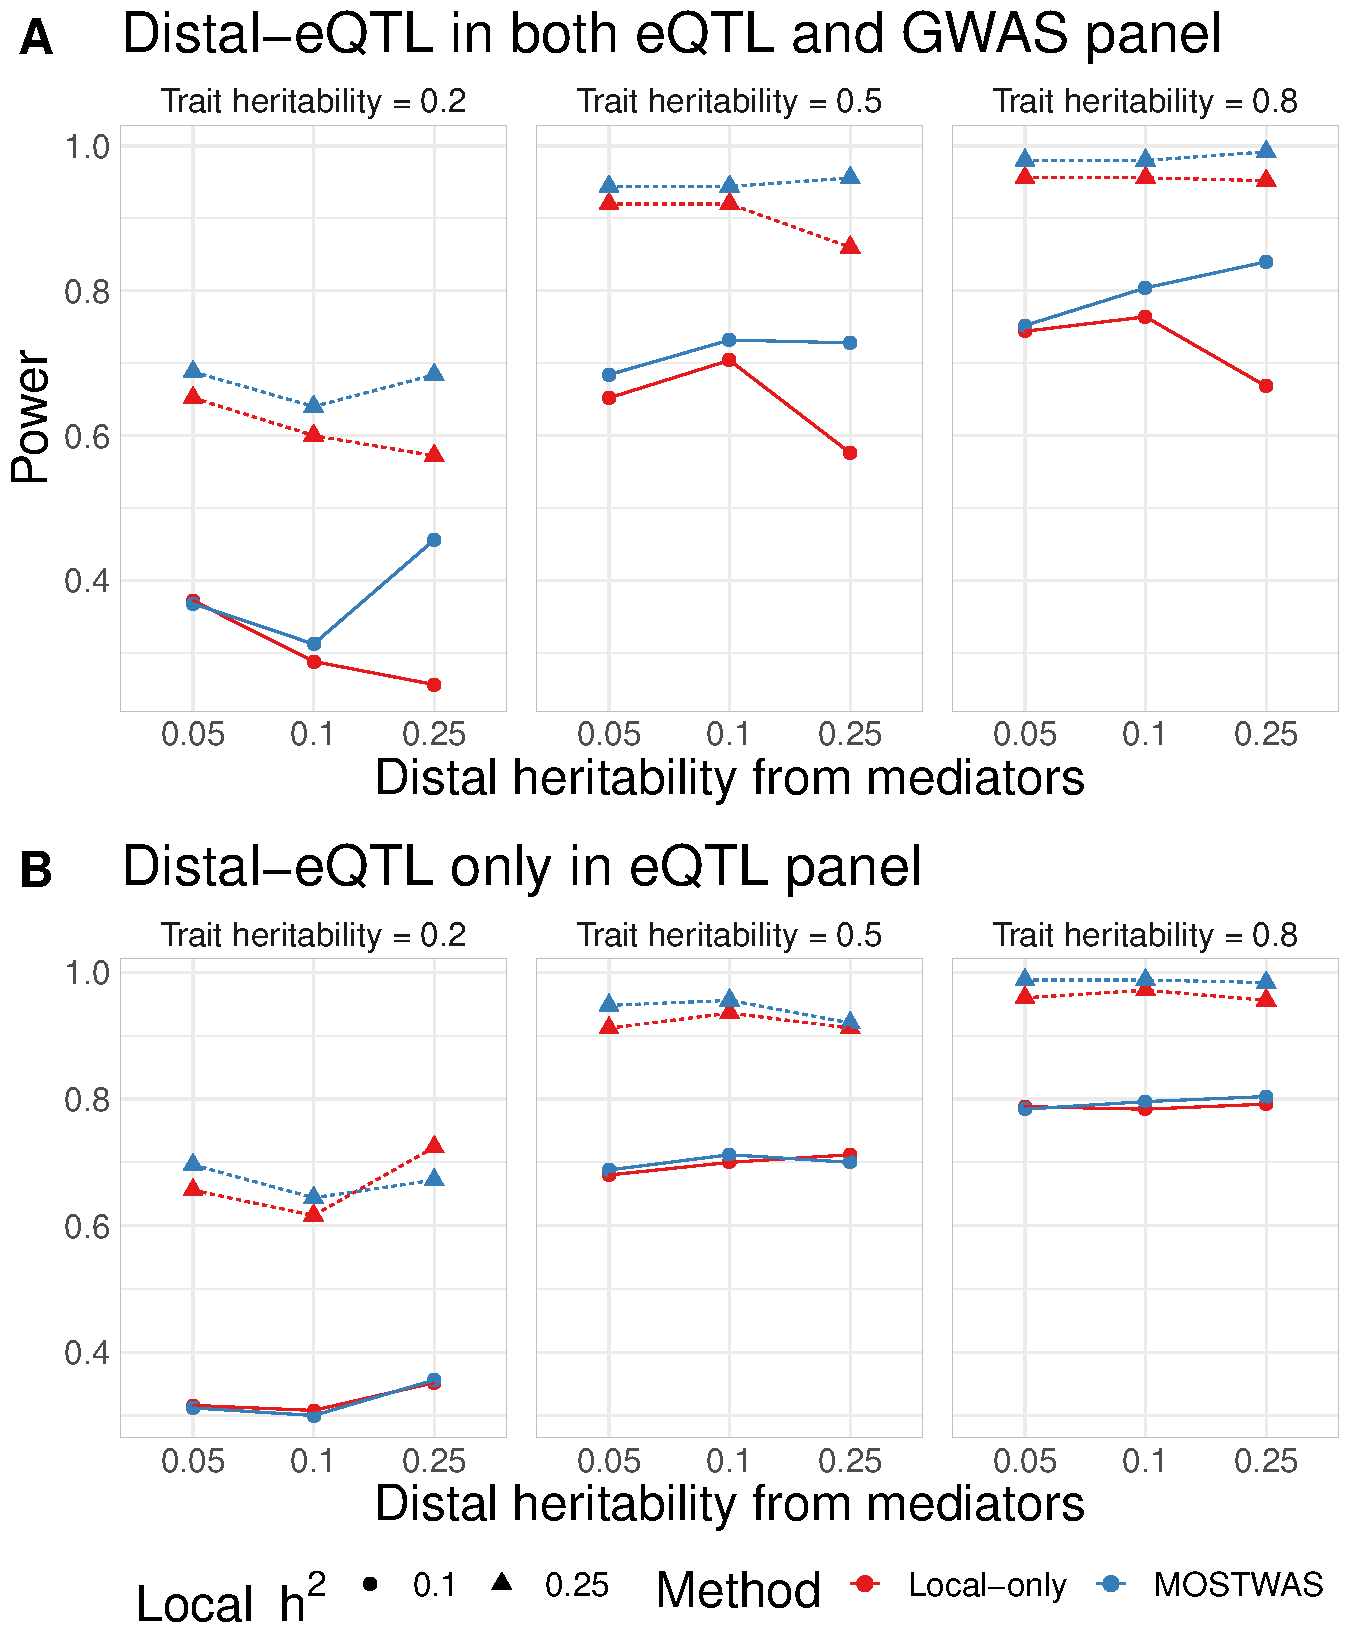
\includegraphics[width = .7\textwidth]{figures/ch4_fig3.pdf}
	\caption{\emph{Comparison of
	TWAS power via simulations
	using MOSTWAS and local-only models.} (A)
	Proportion of gene-trait associations
	at $P < 2.5 \times 10^{-6}$ using local-only (red)
	and the most predictive MOSTWAS (blue) models
	across various local and distal expression heritabilities,
	trait heritability, and causal proportions. (B)
	Proportion of significant gene-trait associations
	across the same simulation parameters with
	no distal effect on the trait in the simulated 
	external GWAS panel.}
	\label{fig:ch4_fig3}
\end{figure}

\subsection{Real data application in breast cancer tumors}

We applied MOSTWAS in the context
of breast tumor multi-omics and
disease outcomes, motivated by recent
GWAS and TWAS into breast cancer-specific survival \cite{Khan2018,Michailidou2013,Michailidou2015,Guo2015,Bhattacharya2020APopulations}. 
Previous breast tumor eQTL studies have
also revealed several signficant
distal-eQTLs in trait-associated
loci, many of which are in regulatory
or epigenetic hotspots
\cite{Bhattacharya2020APopulations,Quiroz-Zarate2017ExpressionTissue},
motivating our application of MOSTWAS
for breast tumor expression modeling.
Using TCGA-BRCA datasets comprising germline SNPs,
tumor mRNA expression, DNA methylation, and miRNA
expression, we trained MeTWAS,
DePMA, and traditional local-only predictive models 
for the mRNA expression of all genes
with germline heritability $h^2 > 0$
at $P < 0.05$.
Estimates of heritability
for genes were considerably larger
when we considered distal variation
using MOSTWAS methods 
(mean heritabilities in \textbf{Supplemental
Table \ref{tbl:ch4_supptab1}}).
We also found that MeTWAS and DePMA
perform better in cross-validation
$R^2$,
with larger numbers of 
models at $R^2 \geq 0.01$
and significant germline heritability
at raw $P < 0.05$
using MOSTWAS methods than
local-only models (\textbf{Figures 
\ref{fig:ch4_fig4}A-C}).
Mean predictive $R^2$
for local-only models was
0.011 (25\% to 75\% inter-quartile
interval (0.0,0.013)), for
MeTWAS models was
0.028 (0.013, 0.032),
and for DePMA models was
0.051 (0.019, 0.068).

In addition to cross-validation,
we used 351 samples in TCGA-BRCA
with only genotype and mRNA expression data
that were not used in model training to
test the portability
of MOSTWAS models in independent
external cohorts. As shown in
\textbf{Figure \ref{fig:ch4_fig5}A and
Supplementary Figure \ref{fig:ch4_suppfig3_5}},
DePMA models obtain the highest
predictive adjusted $R^2$ in
the external cohort (mean 0.016, 25\% to 75\% inter-quartile
interval (0.003, 0.018)), 
with local-only
models (0.013, (0.00,0.013))
outperforming MeTWAS models (0.011,
(0.002, 0.012)),
considering only genes that attained
cross-validation adjusted $R^2 \geq 0.01$
using a given method. Overall,
among genes with cross-validation
adjusted $R^2 \geq 0.01$, 37 out of 280 genes achieved
external predictive $R^2 \geq 0.01$
using local-only models, 89 out of 709 using
MeTWAS, and 787 out of 1,185 using DePMA
(\textbf{Figure \ref{fig:ch4_fig4}A-C}).

Lastly, we conducted association studies
for breast cancer-specific survival
using local-only and the MOSTWAS model with largest
$R^2$ trained
in TCGA-BRCA and summary-level GWAS
data from iCOGs.
Here, we constructed the weighted
burden test, as described above and in Pasaniuc
\etal{} and Gusev \etal{}
\cite{Pasaniuc2014FastEnrichment,Gusev2016}.
We prioritized genes with 
Benjamini-Hochberg \cite{Benjamini1995} adjusted $P < 0.05$
for permutation testing.
Of the 122 genes
that had cross-validation $R^2 \geq 0.01$
in TCGA-BRCA using both local-only
and MOSTWAS models, we found 2 survival
associations with the same loci 
at Benjamini-Hochberg FDR-adjusted 
$0.05$ using both local-only
and MOSTWAS models,
with the strength
of association marginally larger with
the MOSTWAS model in each case (\textbf{Supplemental Figure
\ref{fig:ch4_suppfig2}}).
Furthermore, we find that 116 of these loci
showed larger strengths of association
with survival using the MOSTWAS model
than the local-only model (\textbf{Supplemental Figure
\ref{fig:ch4_suppfig2}}).
QQ-plots for TWAS $Z$-statistics
are provided in \textbf{Supplemental Figure
\ref{fig:ch4_suppfig3}B}
for both local-only and MOSTWAS models.
These results in TCGA-BRCA demonstrated the improved
transcriptomic prediction and power
to detect gene-trait associations using MOSTWAS
over local-only modeling.

\subsubsection{Functional hypothesis
generation with MOSTWAS}

We next conducted TWAS
for breast cancer-specific 
survival using all genes
with significant germline
heritability at $P < 0.05$
with the MOSTWAS model with larger
cross-validation $R^2 > 0.01$.
We identified 21 survival-associated loci
at Benjamini-Hochberg FDR adjusted $P < 0.05$
Of these 21 loci, 11 
persisted when subjected to permutation
testing at a significance threshold of FDR-adjusted $P < 0.05$
(\textbf{Figure \ref{fig:ch4_fig5}C}
and \textbf{Supplemental Table \ref{tbl:ch4_supptab11}}).

An advantage of MOSTWAS is its ability
to aid in functional hypothesis generation
for mechanistic follow-up studies.
The added-last test allows users to
identify genes where trait association
from distal variation is significant above and beyond the
contribution of the local component.
For 8 of the TWAS-associated 11 loci, at
FDR-adjusted $P < 0.05$,
we found significant distal variation added-last
associations (see \textbf{Supplemental Methods}
and \textbf{Supplemental Table \ref{tbl:ch4_supptab11}}), 
suggesting that
distal variation may contribute to the gene-trait
association. All 8 of these loci
showed distal association with
the gene of interest mediated through
a set of four transcription factors 
(\textit{NAA50}, \textit{ATP6V1A}, 
\textit{ROCK2}, \textit{USF3}),
all highly interconnected with the critical MAPK
pathway 
\cite{Dorfel2015TheDisease,Lambertz2015BiologyTreatment,Whitton2018VacuolarCancer,Matsubara2016InhibitorsContext,Chang2018ROCKCells,NiGermlineCarcinoma}. 
These regulatory sites 
serve as an example
of how distal genomic regions 
can be prioritized for
functional follow-up studies to elucidate
the mechanisms underlying the SNP-gene-trait
associations.
These results show the
strength of MOSTWAS to detect and prioritize 
gene-trait
associations that are influenced
by distal variation.

\subsection{Real data application in brain tissue}

We also applied MOSTWAS to transcriptomic data 
on samples of prefrontal cortex,
a tissue that has been used previously
in studying neuropsychiatric traits and disorders
with TWAS \cite{Gusev2018,Raj2018IntegrativeSusceptibility}.
There has been ample evidence in brain tissue, especially the prefrontal
cortex, that non-coding variants
may regulate distal genes \cite{Blauwendraat2016ComprehensiveLobe,Gusev2018,Sey2020AProfiles}; 
in fact, an eQTL analysis
by Sng \etal{} found that approximately
20-40\% of eQTLs in the frontal cortex
can be considered trans-acting \cite{Sng2019Genome-wideDataset}. 
Thus,
the prefrontal cortex in the
context of neuropsychiatric disorders provides a prime
example to assess MOSTWAS.
Using ROS/MAP data on germline SNPs,
tumor mRNA expression, DNA methylation, and miRNA
expression, we trained MeTWAS,
DePMA, and traditional local-only predictive models 
for the mRNA expression of all genes
with germline heritability $h^2 > 0$
at $P < 0.05$. Consistent with results
in TCGA-BRCA, estimates of heritability
for genes were considerably larger
when we considered distal variation
using MOSTWAS methods (\textbf{Supplemental Table \ref{tbl:ch4_supptab1}}).
We also find that MeTWAS and DePMA
perform better in cross-validation
$R^2$ than local-only models (\textbf{Figures 
\ref{fig:ch4_fig4}D-F}).
Mean predictive $R^2$
for local-only models was
0.029 (25\% to 75\% inter-quartile
interval (0.0,0.015)), for
MeTWAS models was
0.079 (0.019, 0.082),
and for DePMA models was
0.045 (0.013, 0.037).

In addition to cross-validation,
we used 87 samples in ROS/MAP
with genotype and mRNA expression data
that were not used in model training to
test the portability
of MOSTWAS models in independent
external cohorts. As shown in
\textbf{Figure \ref{fig:ch4_fig5}A and
Supplementary Figure \ref{fig:ch4_suppfig3_5}},
DePMA models obtain the highest
predictive adjusted $R^2$ in
the external cohort (0.042 (25\% quantile 0.009, 75\% quantile 0.057)), 
with MeTWAS models (0.040 (0.010, 0.054)) also outperforming
local-only
models (0.031 (0.007, 0.039)),
considering only genes that attained
cross-validation adjusted $R^2 \geq 0.01$
using a given method. Overall,
among genes with cross-validation
adjusted $R^2 \geq 0.01$, 187 out of 267 genes achieved
external predictive $R^2 \geq 0.01$
using local-only models, 683 out of 911 using
MeTWAS, and 2,135 out of 2,934 using DePMA
(\textbf{Figure \ref{fig:ch4_fig4}D-F}).

We next conducted association tests
for known Alzheimer's disease risk
loci using local-only and the best MOSTWAS model
(comparing MeTWAS and DePMA cross-validation $R^2$) 
trained
in ROS/MAP and summary-level GWAS
data from IGAP.
From literature, we identified
14 known common and rare loci of late-onset
Alzheimer's disease
\cite{Lambert2013Meta-analysisDisease,Reitz2014GeneticDisease,Sims2017RareDisease,Yuan2017TheDisease},
11 of which had MOSTWAS models
with cross-validation $R^2 \geq 0.01$.
Five of these 11
loci 
(\textit{APOE}, \textit{CLU}, 
\textit{PLCG2}, \textit{SORL1}, 
\textit{ZCWPW1}) showed significant association
at Benjamini-Hochberg FDR-adjusted $P \leq 0.05$
(\textbf{Supplemental Table \ref{tbl:ch4_supptab2}}).
We also compared these 11 associations to
those identified by local-only models
and by latent Dirichlet process regression (DPR)
as implemented in TIGAR \cite{Nagpal2019},
with raw $P$-values of association
shown in \textbf{Figure \ref{fig:ch4_fig5}B}.
MOSTWAS showed stronger associations at 8 of these
loci than both local-only
and DPR models. We followed up on
the 5 significantly associated loci
using the permutation
and added-last tests (see \textbf{Methods} and
\textbf{Supplemental Materials}).
Three of these loci 
(\textit{APOE}, \textit{SORL1}, \textit{ZCWPW1})
showed significant associations, conditional
on large GWAS effect sizes (permutation test 
significant at FDR-adjusted $P < 0.05$)
These three 
loci also showed significant associations with
distal variants, given the association with
local variants, at FDR-adjusted $P < 0.05$ (\textbf{Supplemental 
Table \ref{tbl:ch4_supptab2}}).

We then conducted a transcriptome-wide
association study for risk of major
depressive disorder (MDD) using
summary statistics from the Psychiatric
Genomics Consortium (PGC) genome-wide meta-analysis
that excluded data from the UK Biobank and 
23andMe \cite{Wray2018Genome-wideDepression}.
QQ-plots for TWAS $Z$-statistics
are provided in \textbf{Supplemental Figure
\ref{fig:ch4_suppfig3}B}
for both local-only and MOSTWAS models.
Overall, using all heritable genes with
cross-validation $R^2$ with the best MOSTWAS model
in ROS/MAP, we identified 102 MDD risk-associated loci
with FDR-adjusted $P < 0.05$
 that persisted when subjected to permutation
testing at an FDR-adjusted significance threshold of $P < 0.05$
(colored red in \textbf{Figure \ref{fig:ch4_fig5}D}).
We downloaded genome-wide
association study by proxy (GWAX) summary statistics
from the UK Biobank \cite{Liu2017Case-controlDisease} for replication
analysis of loci identified
using PGC summary statistics. We found that 7
of these 102 loci (labelled
in \textbf{Figure \ref{fig:ch4_fig5}D}) also show an association in UK Biobank
GWAX that is in the same
direction as in PGC.
In comparison,
using local-only models,
we identified 11 genes
with significant association
with MDD risk at FDR-adjusted $P < 0.05$
that persisted permutation testing;
however, none of these loci
showed significant associations
in the UK Biobank GWAX
in the same direction as in PGC.
Summary statistics for MOSTWAS associations
in PGC and UK Biobank are provided 
in \textbf{Supplemental Table \ref{tbl:ch4_supptab3}}.
Local-only results are provided in \textbf{Supplemental
Data}.
It is important to note the UK Biobank dataset is not a GWAS 
dataset as it defines
a case of MDD as any 
subject 
who has the disorder or a first-degree relative 
with MDD, leading to lower power
to detect associations in this
dataset. Nonetheless, we believe that  
strong prediction
of predictive models in independent
cohorts and TWAS results across
two independent cohorts provides
an example of the robustness
of models using MOSTWAS.

\begin{figure}[htbp]
	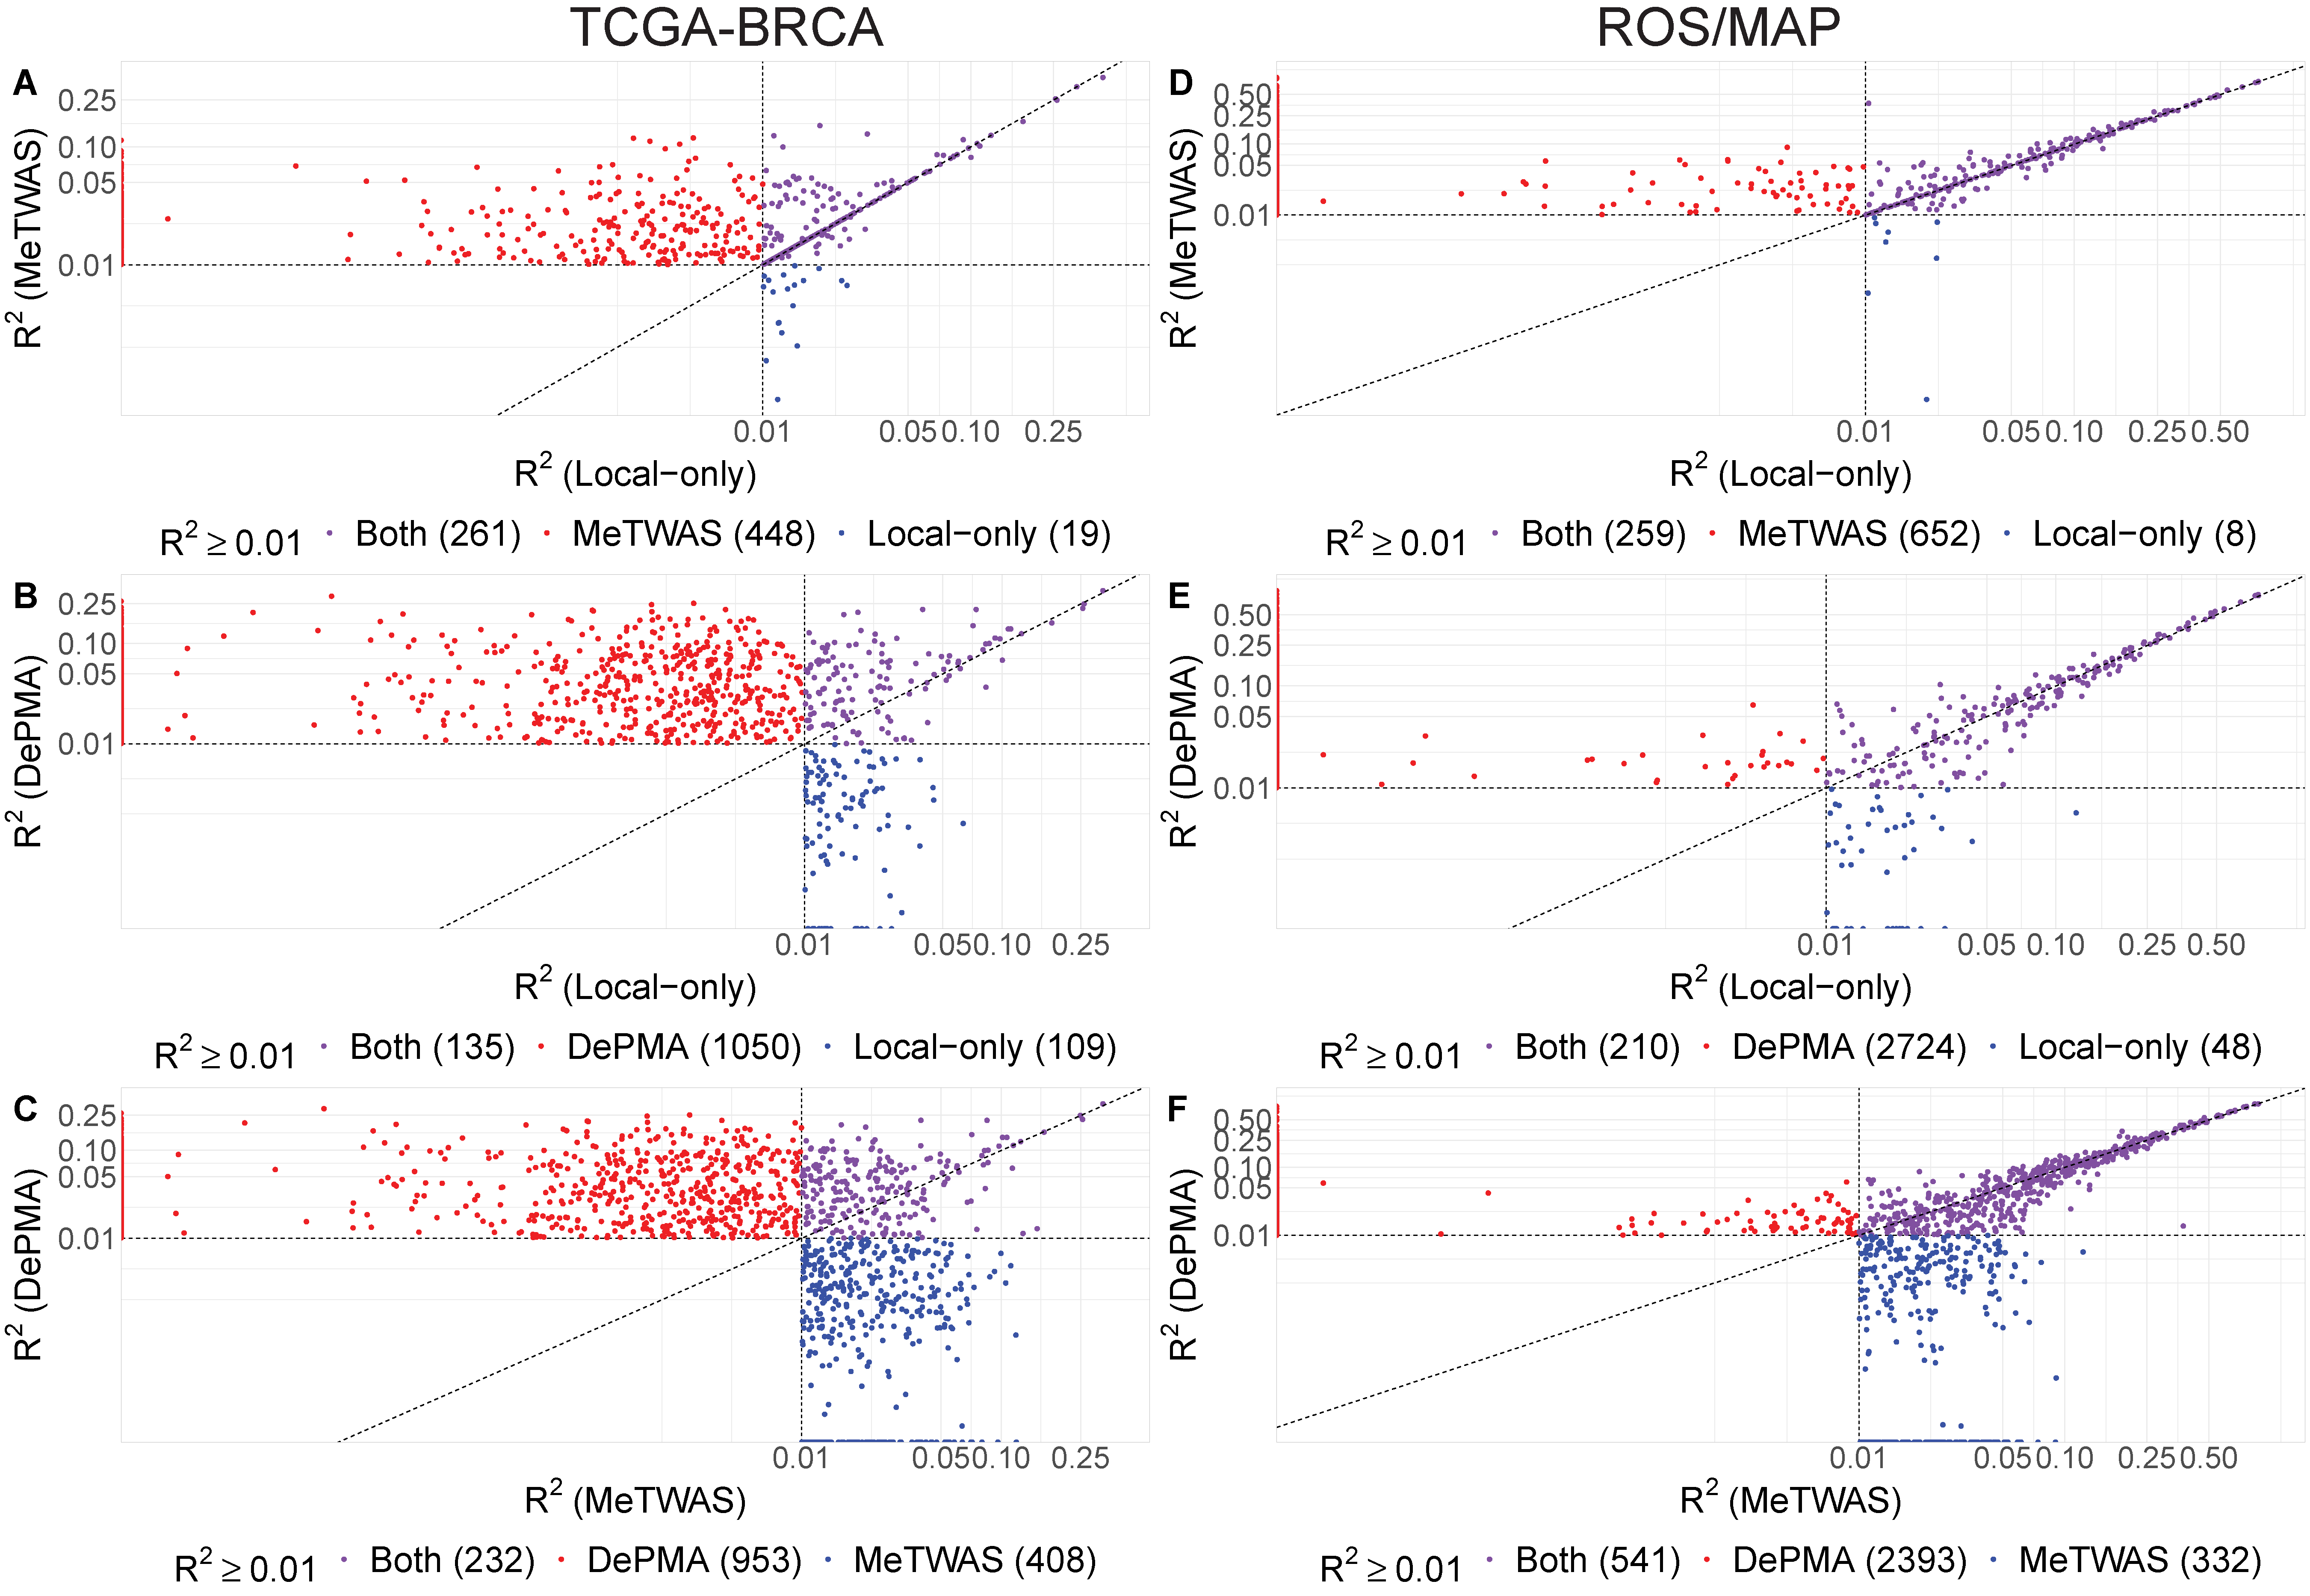
\includegraphics[width = \textwidth]{figures/ch4_fig4.pdf}
	\caption{\emph{Predictive adjusted $R^2$ 
	from cross-validation across
	local-only, MeTWAS, and DePMA
	models.} If a given gene
	does not have $h^2 > 0$
	with $P < 0.05$, we set
	the predictive adjusted $R^2$
	to 0 here for comparison.
	We compare local-only and MeTWAS
	in TCGA-BRCA (A) and ROS/MAP (D),
	local-only and DePMA in TCGA-BRCA (B)
	and ROS/MAP (E), and MeTWAS and DePMA
	in TCGA-BRCA (C) and ROS/MAP (F), all axes indicating the CV
        adjusted $R^2$ for different models.}
	\label{fig:ch4_fig4}
\end{figure}

\begin{figure}[htbp]
	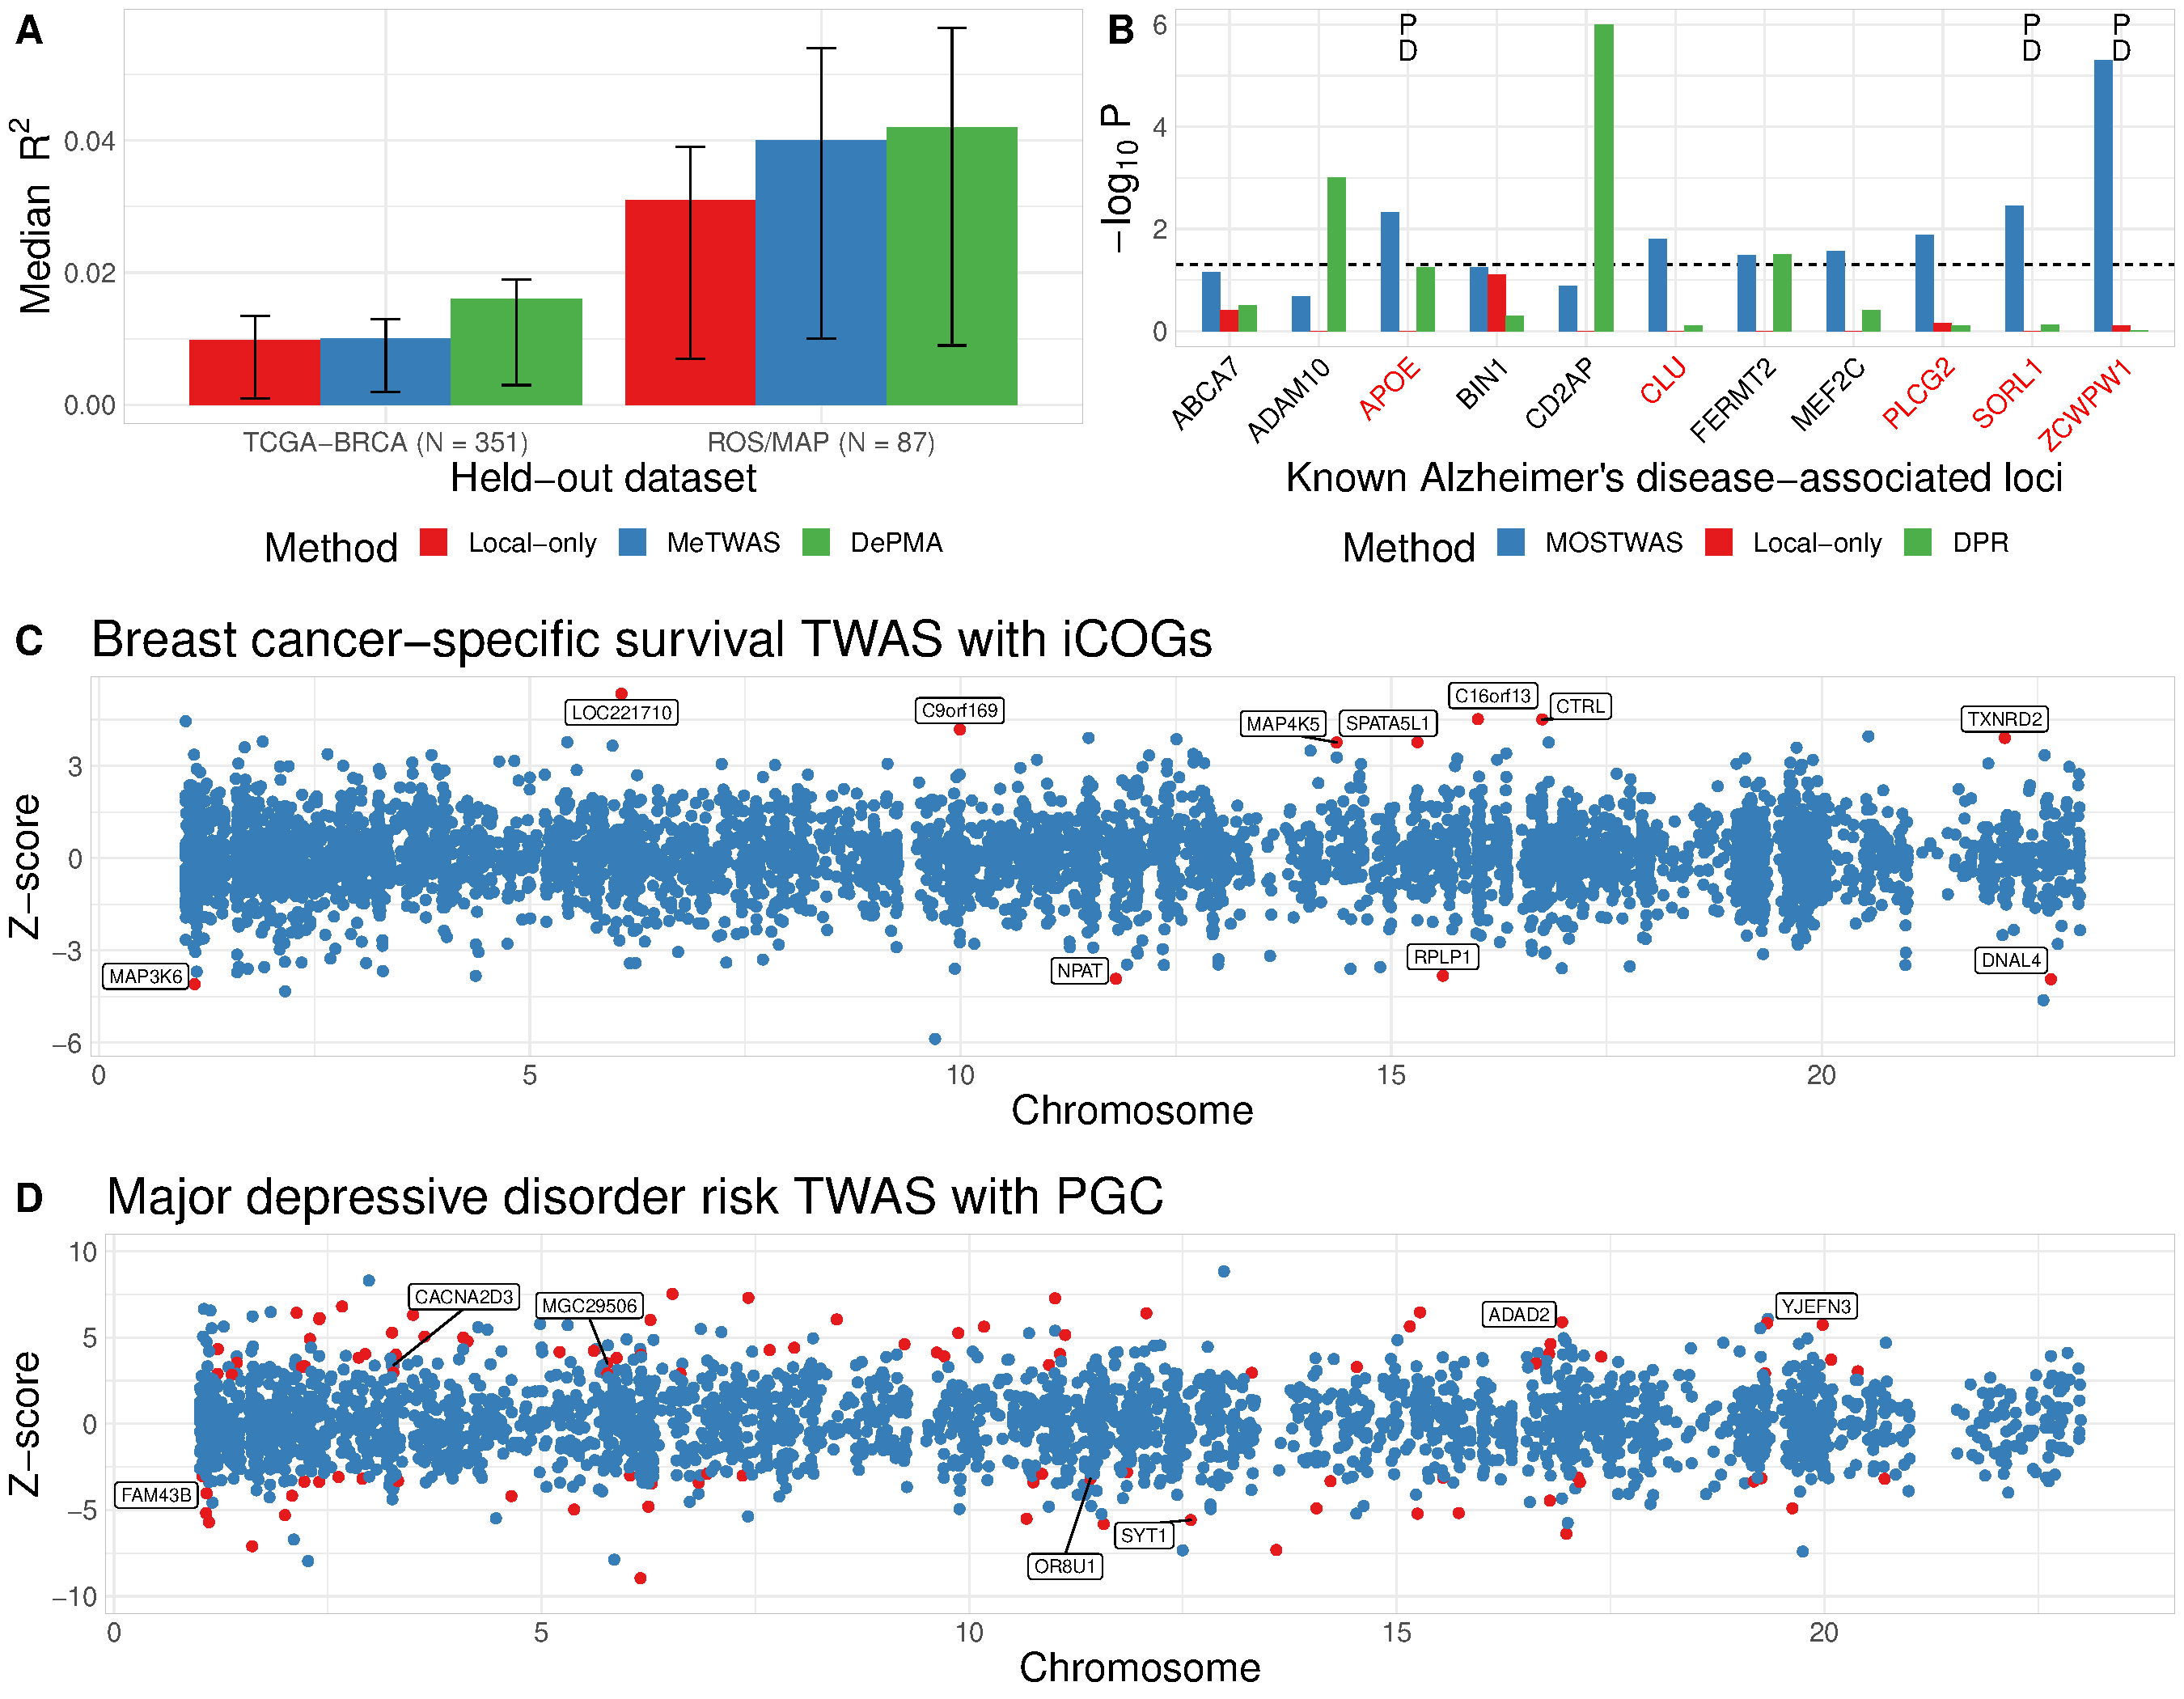
\includegraphics[width = \textwidth]{figures/ch4_fig5.pdf}
	\caption{\emph{External validation of MOSTWAS
	and gene-trait associations
	using MOSTWAS models.} (A) Median predictive
	adjusted $R^2$ in held-out cohorts
	from TCGA-BRCA and ROS/MAP in local-only,
	MeTWAS, and DePMA models that have in-sample significant
	heritability. The interval
	shows the 25\% and 75\% quantiles for external cohort
	predictive $R^2$.
	(B) Associations with 11 known Alzheimer's risk lock,
	as identified in literature, using MOSTWAS, local-only,
	and TIGAR Dirichlet process regression (DPR). (C) TWAS
	associations for breast cancer-specific survival using
	GWAS summary statistics from iCOGs. Loci are colored and
	labelled if the overall association achieves FDR-adjusted 
	$P < 0.05$. Loci
	are labelled with `P' if the permutation test achieves FDR-adjusted $P < 0.05$ and `D' if the added-last
	test achieves FDR-adjusted $P < 0.05$.
	(D) TWAS
	associations for major
	depressive disorder risk using
	GWAS summary statistics from PGC. 
	Loci are colored red if the overall association achieves FDR-adjusted 
	$P < 0.05$ and the permutation test also achieves FDR-adjusted $P < 0.05$.
	We label the 7 loci that
	were independently validated
	with UK Biobank GWAX summary
	statistics at FDR-adjusted
	$P < 0.05$ 
	for both the overall association test
	and permutation test.}
	\label{fig:ch4_fig5}
\end{figure}


We observed that MOSTWAS models generally had 
higher predictive $R^2$ than local-only
models both in training and independent
cohorts. We also found that MOSTWAS
has recapitulated 5 known Alzheimer's
risk loci that were not detected
by local-only modeling (both PrediXcan \cite{Gamazon2015} 
and TIGAR \cite{Nagpal2019}),
3 of which had significant distal associations
using our added-last test.
We also
illustrated that the MOSTWAS detected
MDD-risk loci that were replicable across independent
GWAS and GWAX 
cohorts \cite{Wray2018Genome-wideDepression,Liu2017Case-controlDisease}.

\subsection{Comparison
of computational time}

To assess the difference in computational burden
between local-only, MeTWAS, and
DePMA modelling, we randomly selected a set of 50 genes
that are heritable across all three models
from TCGA-BRCA and computed per-gene
time for fitting using a 24-core, 3.0
GHz processor. We found that 
MeTWAS (mean of 225 seconds
per gene) and DePMA (mean 312 seconds
per gene) took approximately 6-10 times
longer to fit than a traditional local-only model
(mean 36 seconds) 
(\textbf{Supplemental Figure \ref{fig:ch4_suppfig0}}).
Model-fitting here includes heritability
estimation, estimating the SNP-expression
weights, and cross-validation.
We have implemented parallel options
to train an expression model for a single gene 
in MOSTWAS. We also recommend fitting an entire
set of genes from an RNA-seq panel 
via a batch computing
approach \cite{Bischl2015,KoSter2012GenomeEngine}.
Using parallel implementation with 5 cores
and batch computing, we analyzed
15,568 genes from TCGA-BRCA
in approximately 28 hours.